\documentclass[12pt,a4paper]{article}
\usepackage[utf8]{inputenc}
\usepackage[brazil]{babel}
\usepackage{graphicx}
\usepackage{amssymb, amsfonts, amsmath}
\usepackage{float}
\usepackage{enumerate}
\usepackage[top=1.5cm, bottom=1.5cm, left=1.25cm, right=1.25cm]{geometry}

\newcommand{\sen}{\,\textrm{sen}\,}
\newcommand{\arcsen}{\,\textrm{arcsen}\,}
\newcommand{\tg}{\,\textrm{tg}\,}
\newcommand{\arctg}{\,\textrm{arctg}\,}

\begin{document}
\pagestyle{empty}

\begin{center}
  \begin{tabular}{ccc}
    \begin{tabular}{c}
      
\includegraphics[scale=0.25]{../../biblioteca/imagem/brasao-de-armas-brasil} \\
    \end{tabular} & 
    \begin{tabular}{c}
      Ministério da Educação \\
      Universidade Federal dos Vales do Jequitinhonha e Mucuri \\
      Faculdade de Ciências Sociais, Aplicadas e Exatas - FACSAE \\
      Departamento de Ciências Exatas - DCEX \\
      Disciplina: Cálculo Diferencial e Integral I \quad Semestre: 2021/2\\
      Prof. Me. Luiz C. M. de Aquino\\
    \end{tabular} &
    \begin{tabular}{c}
      
\includegraphics[scale=0.25]{../../biblioteca/imagem/logo-ufvjm} \\
    \end{tabular}
  \end{tabular}
\end{center}

\begin{center}
  \textbf{Lista II}
\end{center}

\begin{enumerate}
 \item Calcule a derivada das funções definidas abaixo.

 \begin{tabular}{llll}
  (a) $f(x) = x^2\cos x$  & (c) $u(a) = \left(1 - \dfrac{1}{a}\right)\cos a$ & (e) $j(u) = \cos^2 u - \sen^2 u$ & (g) $h(s) = \ln\dfrac{1}{s}$\\
  & \\
  (b) $g(t) = \dfrac{1 - t^2}{1 + \sen t}$  & (d) $v(r) = \dfrac{e^r - r^2}{r^3 + r}$ & (f) $w(k) = \left(1 - 3k^4\right)^5$ & (h) $i(v) = 2^{v^3 - 1}$
 \end{tabular}
 
 \item Determine a reta tangente ao gráfico das funções definidas abaixo nos pontos indicados.

 \begin{tabular}{ll}
  (a) $f(x) = \dfrac{x-1}{x+1}$, $P=\left(3;\, \dfrac{1}{2}\right)$. & (c) $g(x) = x^2 \log x$, $P=\left(1;\, 0\right)$.\\
  (b) $h(x) = \dfrac{\sen x}{x}$, $P=\left(\pi;\, -\dfrac{1}{\pi}\right)$. & (d) $j(x) = \cos x e^x$, $P=\left(0;\, 1\right)$.
 \end{tabular}
 
  \item  Em um jogo de naves espaciais, considere que a nave se movimenta ao
longo do gráfico da função $f(x)=\dfrac{1}{4}x^{2}-3x+10$. Além disso,
ao disparar um projétil, ele seguirá a trajetória da reta tangente
ao gráfico de $f$ na posição em que a nave está, como ilustra a figura
abaixo. Nessas condições, se a nave está no ponto $(3,\, f(3))$,
então o projétil atingirá o solo (eixo $x$) em que posição?

\begin{figure}[H]
\centering
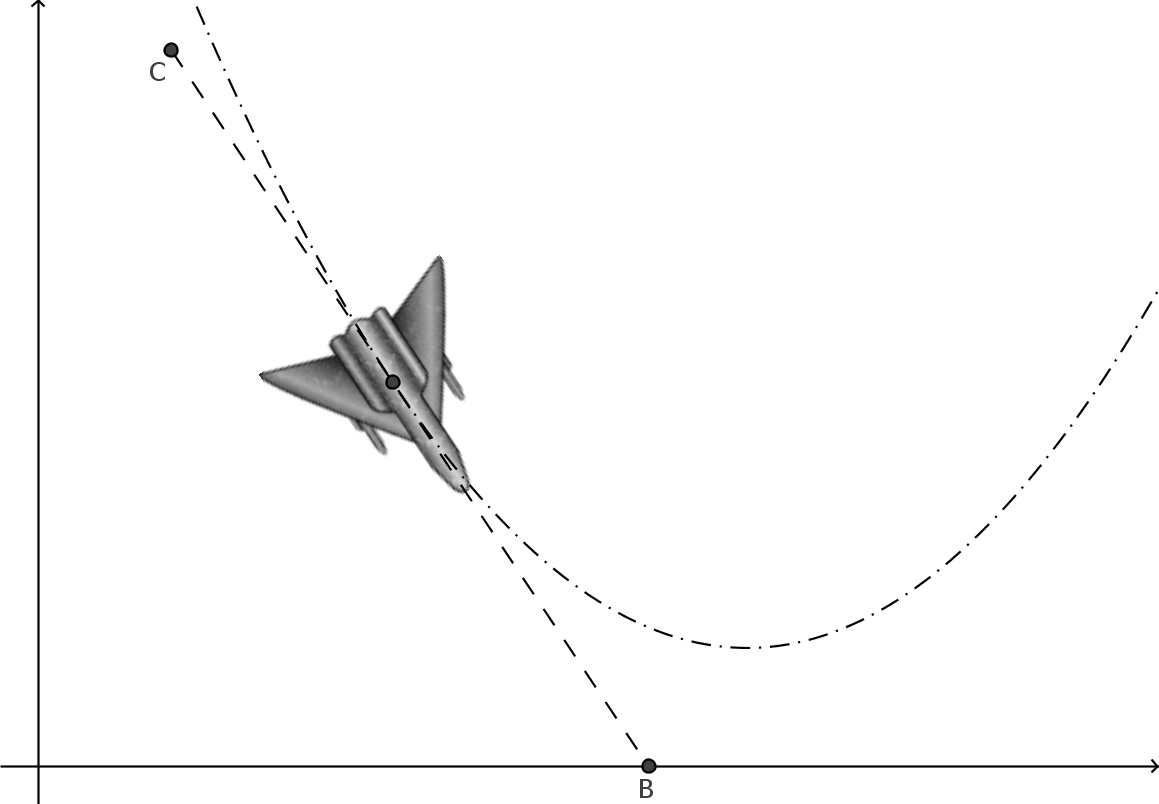
\includegraphics[scale=0.7]{imagem/nave-espacial.png}
\end{figure}
  
  \item Usando o fato de que $[\cos x]^\prime = -\sen x$, exiba um desenvolvimento para justificar que 
$[\arccos x]^\prime = -\dfrac{1}{\sqrt{1 - x^2}}$.

  \item Usando o fato de que $[\sen x]^\prime = \cos x$, exiba um desenvolvimento para justificar que 
$[\arcsen x]^\prime = \dfrac{1}{\sqrt{1 - x^2}}$.
\end{enumerate}

\newpage
\begin{center}
  \textbf{Gabarito}
\end{center}

\textbf{[1]} 
(a) $f^\prime(x) = -x^2\sen x + 2x\cos x$. (b) $g^\prime(t) = \dfrac{t^2\cos t  - 2t\sen t - 2t - \cos t}{(1 + \sen t)^2}$. 

(c) $u^\prime(a) = -\dfrac{a^2\sen a - a\sen a - \cos a}{a^2}$. (d) $v^\prime(r) = \dfrac{r^4 + r^3e^r - 3r^2e^r - r^2 + re^r - e^r}{(r^3 + r)^2}$. 

(e) $j^\prime(u)=- 2\sen 2u$. (f) $w^\prime(k) = -60k^3\left(1 - 3k^4\right)^4$. 

(g) $h^\prime(s) = -\dfrac{1}{s}$. (h) $i^\prime(v) = (3\ln 2)2^{v^3 - 1}v^2$. 

\textbf{[2]} (a) $y = \dfrac{1}{8}x + \dfrac{1}{8}$. (b) $y = -\dfrac{1}{\pi}x  + \dfrac{\pi - 1}{\pi}$. 

(c) $y = \dfrac{1}{\ln 10}x  - \dfrac{1}{\ln 10}$. (d) $y = x + 1$. 

\textbf{[3]} Posição: $B=(\frac{31}{6},\,0)$. 

\textbf{[4]} Sugestão: comece calculando $\left[\cos\left(\arccos x\right)\right]^\prime=[x]^\prime$.

\textbf{[5]} Sugestão: comece calculando $\left[\sen\left(\arcsen x\right)\right]^\prime=[x]^\prime$.
\end{document}